\chapter{Work Progress}
\label{chap:work}
\setlength{\parskip}{1.5mm}
%\setlength{\baselineskip}{1.4mm}
\section{Verifying the Algorithm in MATLAB}
\subsection{Model of Non-Linear Dynamic System}
A schematic diagram of the compound triple-pendulum system is shown in Figure 5.1.The bars of the pendulum have significant mass so that it can be modeled as a compound pendulum. The model has been parameterized according to the physical characteristics of the system including mass of the bars, their inertia etc. 
% Damping factors were also included in the model for higher degree of chaos and non-linearity in the system. 
% Each bar ${i}$ is defined by a set of four parameters: 
% ${I_{i}}$, the moment of inertia of the bar, ${m_{i}}$, the mass of the bar,
%  ${L_{i}}$, the length of the bar, and
%  ${k_{i}}$, the damping coefficient of the bar rotating about it’s upper joint. 
The position and velocity of the bars are defined by the six system state variables: $\theta$\textsubscript{1}, $\theta$\textsubscript{2}, $\theta$\textsubscript{3}, ${\dot{\theta\textsubscript{1}}}$, ${\dot{\theta\textsubscript{2}}}$, ${\dot{\theta\textsubscript{3}}}$

%\begin{figure}
%\centering
%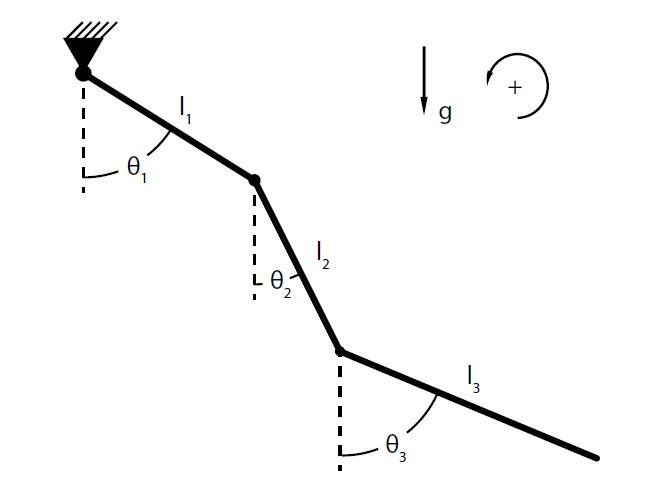
\includegraphics[width=8cm]{pendulum.jpg}
%\caption{Schematic Diagram of Triple Pendulum System}\label{fig:pendulum}
%\end{figure}
% 

\begin{figure}[H]
\begin{subfigure}{0.5\textwidth}
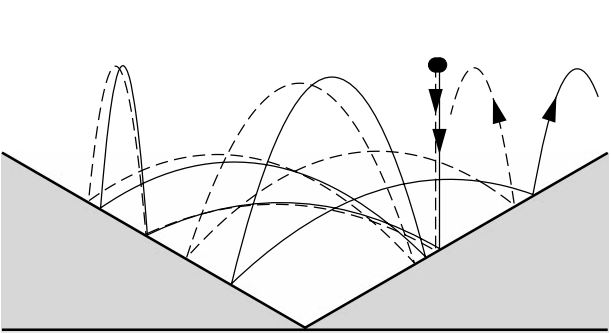
\includegraphics[width=1.1\linewidth]{ball.jpg}
\caption{Chaotic motion of a bouncing ball}\label{fig:ball}
\end{subfigure}
\begin{subfigure}{0.5\textwidth}
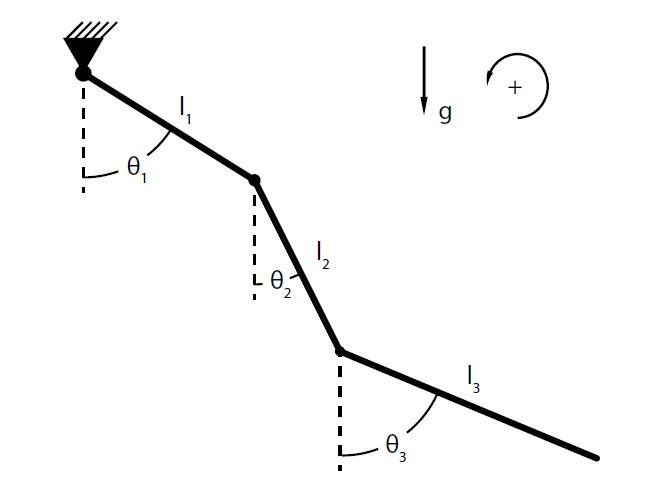
\includegraphics[width=0.8\linewidth]{pendulum.jpg}
\caption{Schematic Diagram of Triple Pendulum}\label{fig:pendulum}
\end{subfigure}
\caption{Examples of Non-Linear Dynamic systems}\label{fig:image1}

\end{figure}
\begin{figure}[h]
\begin{subfigure}{0.5\textwidth}
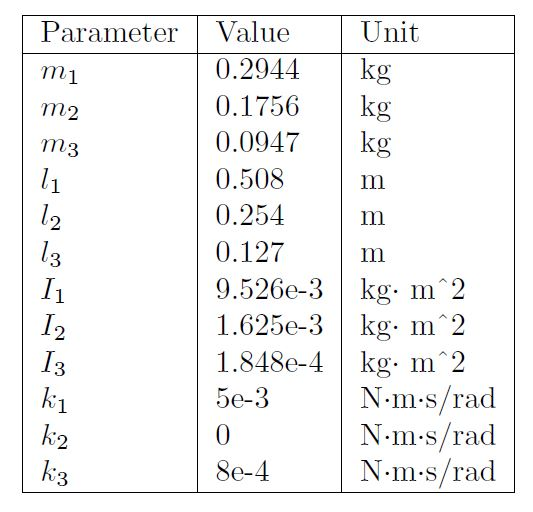
\includegraphics[width=0.8\linewidth]{param.jpg}
\caption{Table 1}\label{fig:param}
\end{subfigure}
\begin{subfigure}{0.5\textwidth}
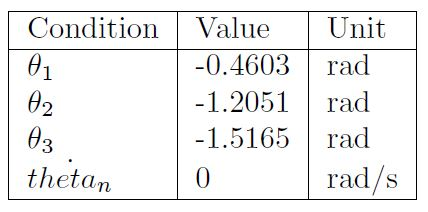
\includegraphics[width=0.8\linewidth]{ic.jpg}
\caption{Table 2}\label{fig:ic}
\end{subfigure}
\caption{Parameters \& Initial Conditions for the Initial Value Problem}\label{fig:image2}
\end{figure}

% \begin{figure}
% 
% 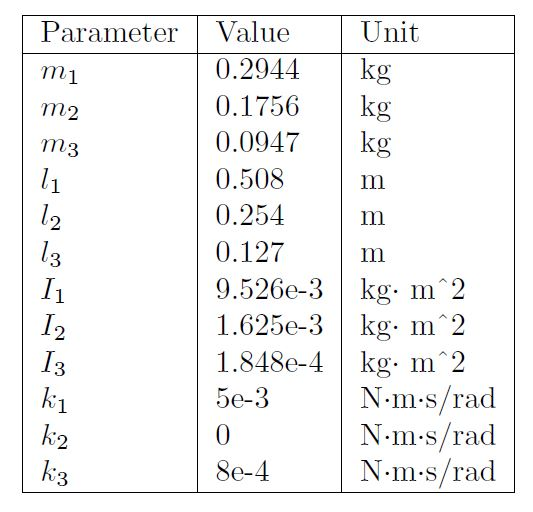
\includegraphics[width=8cm]{param.jpg}
% \caption{Parametric Values used for Simulation}\label{fig:param}
% \end{figure}
% 
% \begin{figure}
% % \centering
% 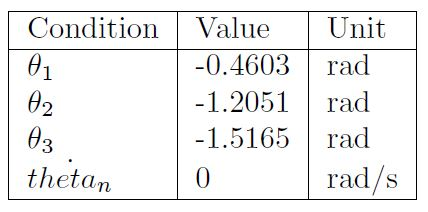
\includegraphics[width=8cm]{ic.jpg}
% \caption{Initial Conditions used for Simulation}\label{fig:ic}
% \end{figure}

\subsection{Simulation of Compound Triple Pendulum}
This compound triple-pendulum model has been simulated using MATLAB using approximate differential equations describing the random motions. The parameters and initial conditions of the ODEs are given in Table 1 and Table 2 respectively. For the simulation, simple numerical methods were used to solve the differential equations and the values corresponding to the angular position of the bars were obtained within a certain duration of time with a predefined precision. This generates the mapping values for the encryption module. 

% \begin{figure}[H]
% \centering
% 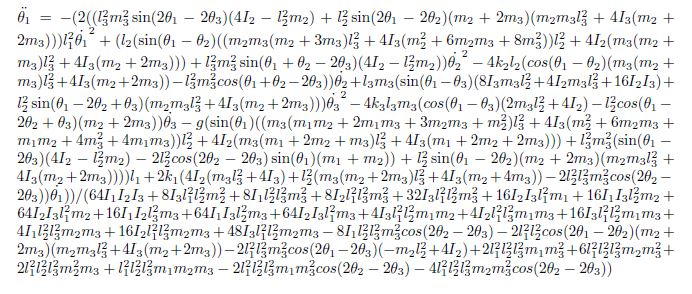
\includegraphics[width=16cm]{diff1.jpg}
% \caption{Differential Equation for ${\theta\textsubscript{1}}$}\label{fig:diff1}
% \end{figure}
% 
% 
% \begin{figure}[H]
% \centering
% 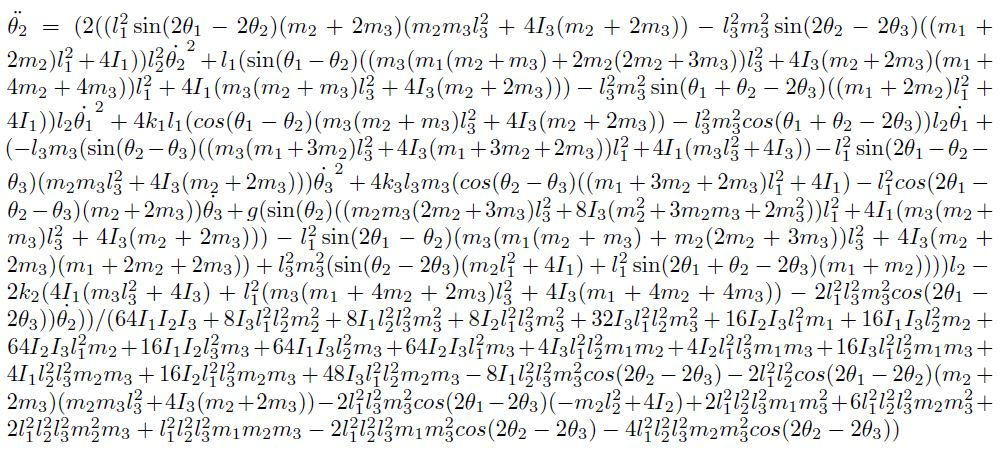
\includegraphics[width=16.5cm]{diff2.jpg}
% \caption{Differential Equation for ${\theta\textsubscript{2}}$}\label{fig:diff2}
% \end{figure}
% 
% 
% \begin{figure}[H]
% \centering
% 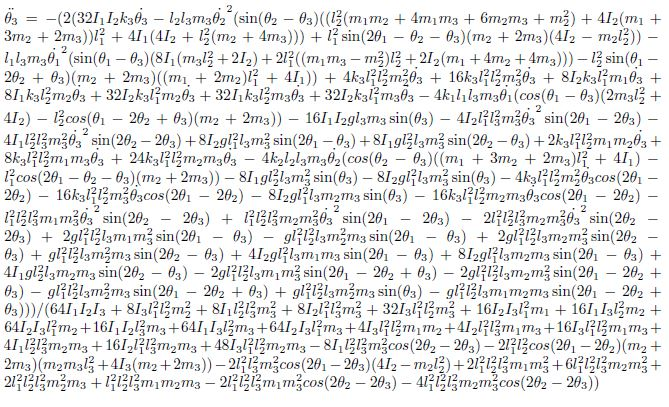
\includegraphics[width=16.5cm]{diff3.jpg}
% \caption{Differential Equation for ${\theta\textsubscript{3}}$}\label{fig:diff3}
% \end{figure}
% \vfill
\subsubsection{Simulation Results}
These are some of the observations from the simulation of the triple-pendulum model for a duration of t = 0 to t = 10 seconds with $\Delta$t = 0.001 :\\
(i) Initial conditions are same as given in Table 1 \& 2:\\
 
\begin{figure}[H]
\begin{subfigure}{0.5\textwidth}
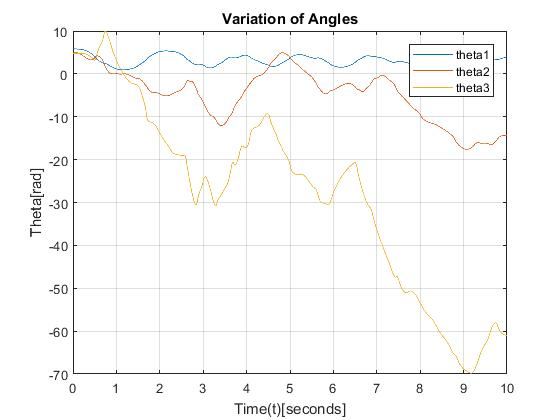
\includegraphics[width=1\linewidth]{theta.jpg}
\caption{Plot of ${\theta}$ vs Time}\label{fig:theta}
\end{subfigure}
\begin{subfigure}{0.5\textwidth}
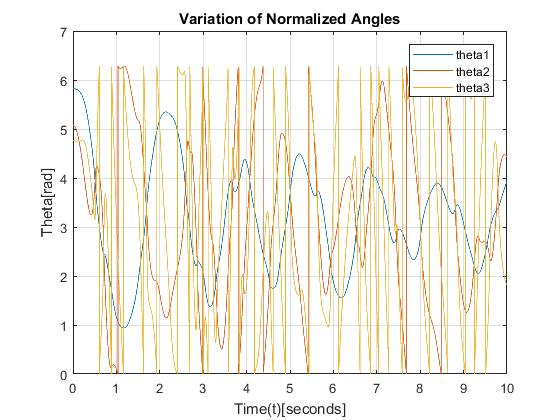
\includegraphics[width=1\linewidth]{theta_norm.jpg}
\caption{Plot of Normalized ${\theta}$ vs Time}\label{fig:theta_norm}
\end{subfigure}
\caption{Motion of Triple-Pendulum for t = 0 to t = 10 sec}\label{fig:image3}
\end{figure}

\begin{figure}[H]
\centering
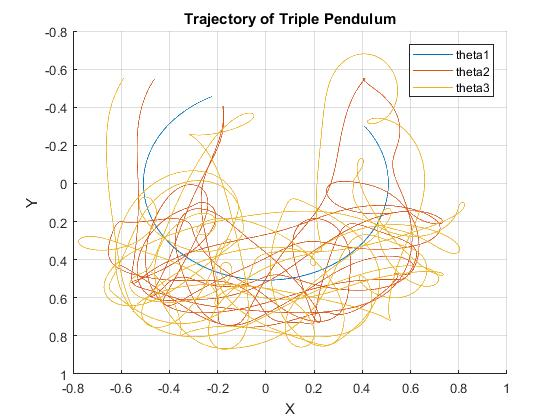
\includegraphics[width=0.7\linewidth]{trajectory.jpg}
\caption{Plot of Motion of Triple-Pendulum}\label{fig:trajectory}
\end{figure}


\subsection{Encryption - Decryption}
Our approach is to convert the plain-text into ascii format and  map the value to the intervals partitioned from the range of values of the triple-pendulum motion simulated within a specific duration of time for a particular set of parameters and initial conditions. The initial conditions and parameters of the different equation forms a part of the private key. Following the Baptista-type method, the entire range of the chaotic function was partitioned into a number of intervals equal to the number of characters. Each character in the plain-text is then mapped to a specific interval and then to a time point randomly selecting from that interval.  

\begin{figure}[H]
\centering
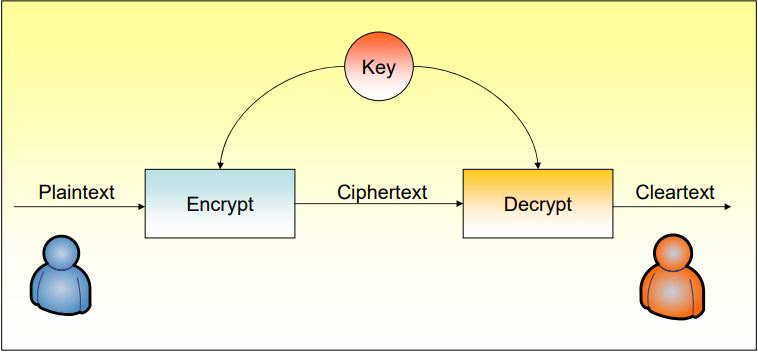
\includegraphics[width=10cm]{crypto.jpg}
\caption{Working Principle of a Symmetric Cryptosystem}\label{fig:crypto}
\end{figure}

On the decryption module, the interval in which the encrypted value lies is computed from the generated motion of the triple-pendulum for the same key and the corresponding index would then refer to the ascii converted clear-text. Converting them into characters, the message can be decoded.\\
\begin{figure}[H]
\centering
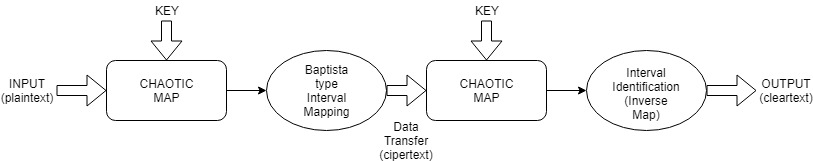
\includegraphics[width=16cm]{Dataflow.jpg}
\caption{Encryption-Decryption Strategy}\label{fig:Dataflow}
\end{figure}


\section{Key Generation}
It is observed that for certain specific parameters or initial conditions, the motion of the bars of the triple-pendulum shows periodic nature after a certain span of time. Hence there is a need to eliminate those parameters or initial conditions for which the motion is periodic as the periodic nature breaks the chaotic behavior of the system. For that a test for periodicity was employed to extract the prominent period of the signal using statistical analysis on the spectrum of the signal. The test used is known as {\bf{\em Fisher's g-statistic test}}(see [11]). This method is based on the test of significance of the periodic components of the signal derived from its periodogram. 

\begin{figure}[H]
\centering
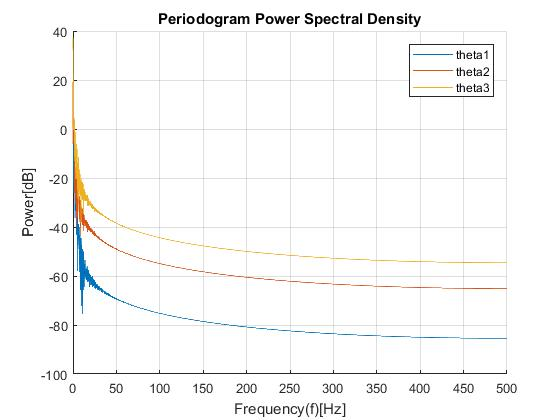
\includegraphics[width=0.7\linewidth]{periodogram.jpg}
\caption{Periodogram Plot for ${\theta}$}\label{fig:periodogram}
\end{figure}


\begin{figure}[H]
\begin{subfigure}{0.5\textwidth}
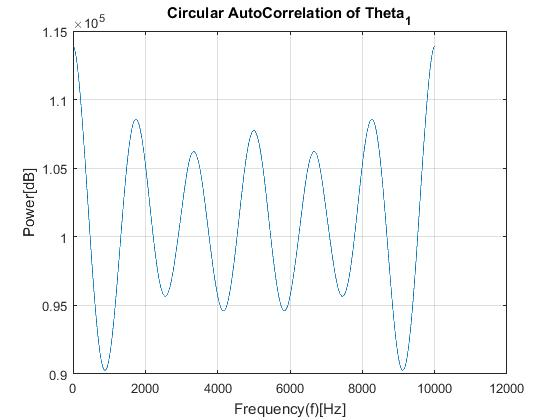
\includegraphics[width=1\linewidth]{auto_corr1.jpg}
\caption{Plot of Circular Auto-Correlation for ${\theta_{1}}$}\label{fig:cir_auto1}
\end{subfigure}
\begin{subfigure}{0.5\textwidth}
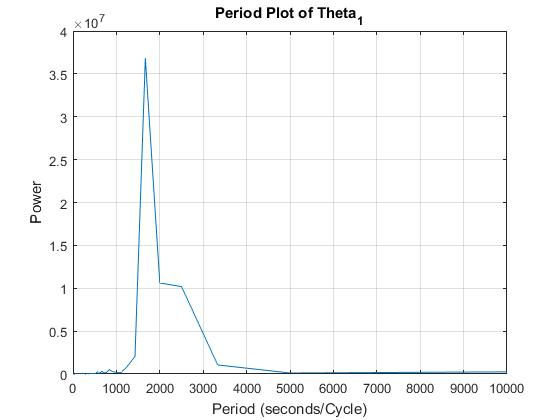
\includegraphics[width=1\linewidth]{period1.jpg}
\caption{Plot of Periodicity for ${\theta_{1}}$}\label{fig:period1}
\end{subfigure}
\caption{Periodic Properties of ${\theta_{1}}$}\label{fig:image4}
\end{figure}

\begin{figure}[H]
\begin{subfigure}{0.5\textwidth}
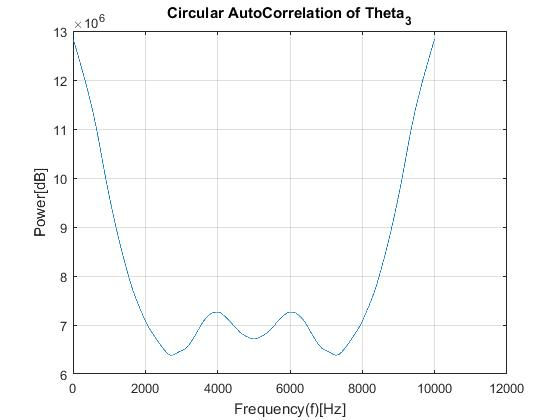
\includegraphics[width=1\linewidth]{auto_corr3.jpg}
\caption{Plot of Circular Auto-Correlation for ${\theta_{3}}$}\label{fig:cir_auto3}
\end{subfigure}
\begin{subfigure}{0.5\textwidth}
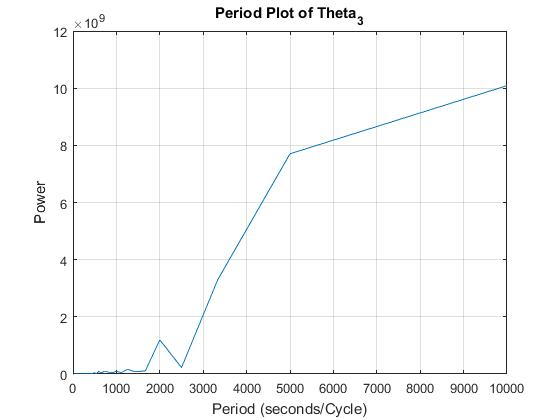
\includegraphics[width=1\linewidth]{period3.jpg}
\caption{Plot of Periodicity for ${\theta_{3}}$}\label{fig:period3}
\end{subfigure}
\caption{Periodic Properties of ${\theta_{3}}$}\label{fig:image5}
\end{figure}

From the figures 5.8 \& 5.9 , it is observed that there is peak at 1700 (seconds/Cycle) for $\theta_{1}$ whereas no such peak occurs for $\theta_{3}$. Thus $\theta_{1}$ is periodic in nature. The values obtained from the periodicity test and plots of circular auto-correlation clearly differentiates the parameters and initial values which leads to periodic nature of the motion and those which lead to non-periodic nature of the motion. Thus by iterating through all possibles values of the parameters and checking likewise for non-periodic nature, a set of keys was generated and stored. 
\\\\\\

\section{FPGA Implementation}
The complete design has been implemented at Register-Transfer Level (RTL) in {\bf SystemVerilog HDL} and the target device chosen is Digilent Nexys Board with {\bf Xilinx Artix-7 FPGA}. The synthesis tool used is Xilinx Synthesis Tool (XST). The following diagram shows the implementation plan for the design :
% \begin{center}
\begin{figure}[H]
\centering
\resizebox{10cm}{10cm}{
\begin{tikzpicture}[->,>=stealth',shorten >=1pt,auto,node distance=5cm, semithick]
  %\tikyle{every state}=[draw=none,text=black]
    
  \node[state] (A)                         {\begin{tabular}{c}$Control$\\$Unit$\end{tabular}};
  \node[state] (C) [above of=A]            {\begin{tabular}{c}$Ethernet$\\$\&$\\$USB$ $ Interface$\\$Module$\end{tabular}};
  \node[state] (B) [right of=C]      {\begin{tabular}{c}$I/O$\\$Ports$\end{tabular}};
  \node[state] (D) [below right of=A]      {\begin{tabular}{c}$LUT2$\\$Mapping$ $of$\\$Plaintext$ $to$\\$Ciphertext$\end{tabular}};
  \node[state] (E) [below left of=A]       {\begin{tabular}{c}$LUT1$\\$Various$\\$Constants$\end{tabular}};
  \node[state] (F) [below of = A]           {\begin{tabular}{c}$Arithmetic$\\$\&$ $Logic$\\$Unit$\end{tabular}};

\path
% (A) edge [loop right] node {} (A)
% (B) edge             node {} (A)
(C) edge             node {} (B)
(D) edge [bend right] node {} (A)
(E) edge [bend left]node {} (A)
(F) edge             node {} (A)
(A) edge             node {} (F)
(A) edge             node {} (C)
(C) edge             node {} (A)
(A) edge [bend right] node {} (D)
(A) edge [bend left]node {} (E);
% \node[below=7cm] at (current bounding box.base) {Overview of FPGA Implementation};
\end{tikzpicture}
}\caption{Overview of FPGA Implementation}\label{fig:fpga_implement}
\end{figure}
% \end{center}




% \begin{figure}[H]
% \centering
% 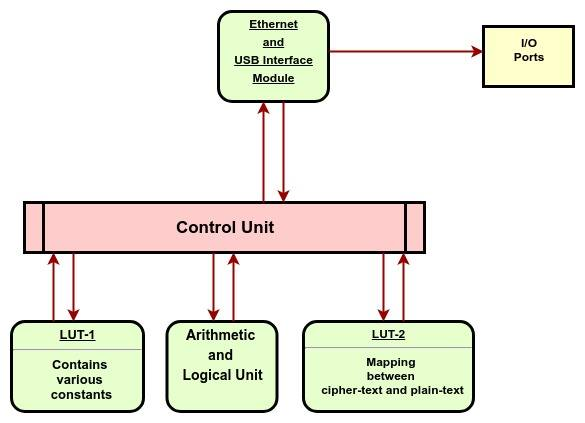
\includegraphics[width=10cm]{fpga_block.jpg}
% \caption{Block Diagram of FPGA Implementation}\label{fig:fpga_block}
% \end{figure}


\subsection{Arithmetic and Logic Unit (ALU)}
The Arithmetic and Logical Unit (ALU) has been appropriately parametrised to enable it to function at any given level of floating point precision (default format is IEEE-754). It consists of the following datapath units -

1. {\bf Addition Module} - This module performs floating point addition. The complete datapath has been split into 4 stages keeping in mind the target clock frequency 100 MHz. Current design contains 2 units of Addition Module.

2. {\bf Multiplication Module} - This module performs floating point multiplication. The complete multiplication datapath has been split into 5 stages in order to achieve the target clock frequency. Moreover, if required, the module can be configured to function in pipeline mode. Current design contains 1 unit of Multiplication Module.
\\

3. {\bf Exponentiation Module} - This module evaluates the value of an input raised to an integer exponent. It utilises an instance of the multiplication module. Current design contains 1 unit of Exponentiation Module.

4. {\bf Division Module} - This module performs floating point division. The complete datapath has been split into multiple stages keeping in mind the target clock frequency 100 MHz. However, since, the division operation requires significantly more clock cycles compared to other operations, the design has been optimised to reduce the number of division oeration to minimum. Current design contains 1 unit of Division Module.

\begin{figure}[H]
\centering
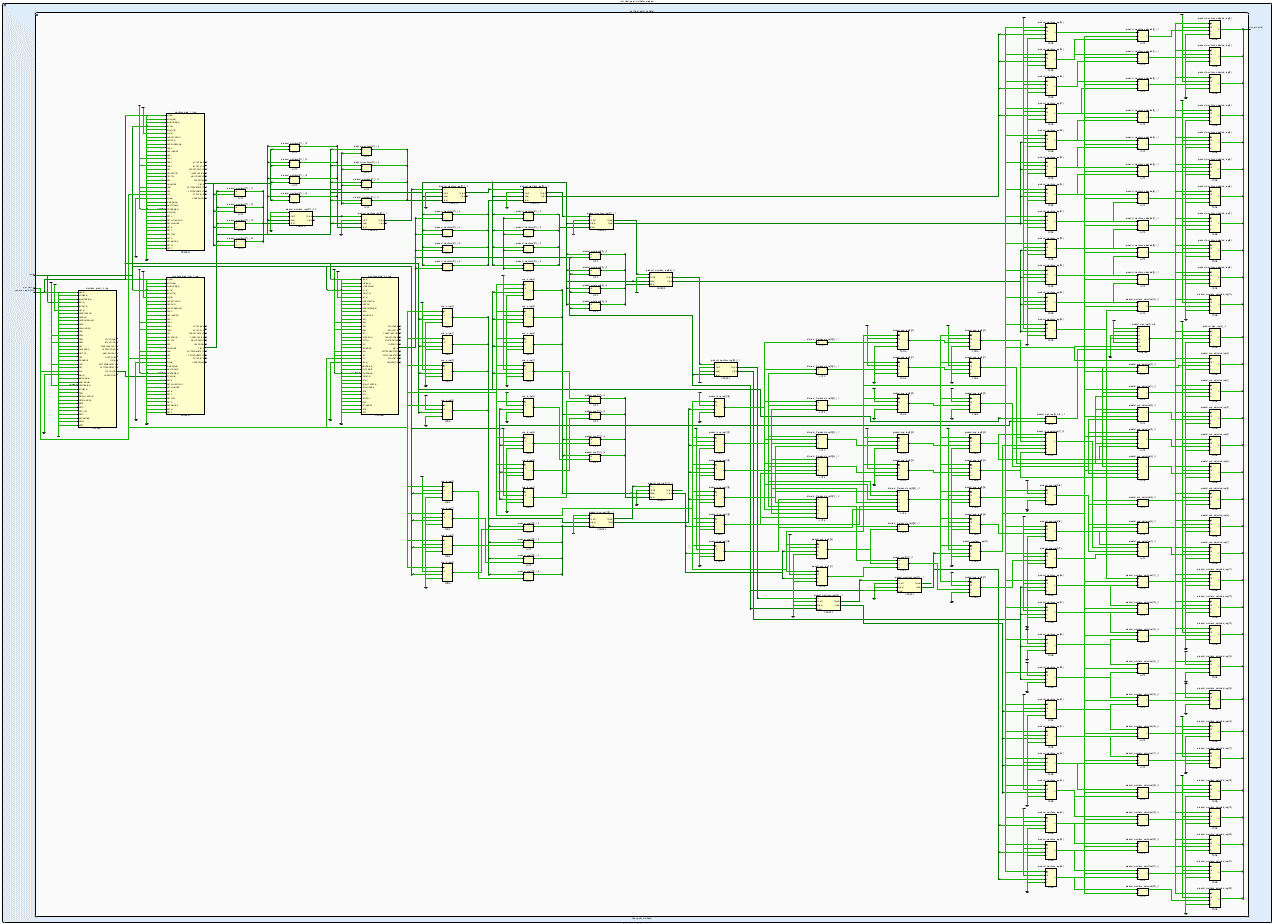
\includegraphics[width=15cm]{schematic.png}
\caption{Schematic of multiplier module}\label{fig:schematic}
\end{figure}

\subsection{Control Unit}
The control unit of the implementation is essentially a Finite State Machine (FSM) which performs the required tasks in a well-defined sequence. In order to achieve an efficient implementation, the complete FSM has been factored into simpler state machines. A top-level FSM serves as control for these simpler FSMs. Basic description for these state machines is given as follows -

\subsubsection{Top-Level State Machine}

% \begin{center}
\begin{figure}[H]
\centering
\resizebox{10cm}{10cm}{
\begin{tikzpicture}[->,>=stealth',shorten >=2pt,auto,node distance=6cm, semithick]
  %\tikyle{every state}=[draw=none,text=black]

  \node[state] (A)                         {$DEFAULT$};
  \node[state] (B) [above left of=A]      {\begin{tabular}{c}$RECEIVE$\\$KEY$\end{tabular}};
  \node[state] (C) [right of=B]            {\begin{tabular}{c}$EVALUATE$\\$EXPRESSION$\end{tabular}};
  \node[state] (D) [below right of=C]      {\begin{tabular}{c}$MODIFY$\\$STATE$\\$VARIABLES$\end{tabular}};
  \node[state] (E) [below left of=D]       {\begin{tabular}{c}$OBTAIN$\\$CHAOTIC$\\$MAP$\end{tabular}};
  \node[state] (F) [left of = E]           {\begin{tabular}{c}$GENERATE$\\$CIPHERTEXT$\end{tabular}};
  %\node[state] (G) [left of = F]           {\begin{tabular}{c}$STORE$\\$CIPHERTEXT$\end{tabular}};

\path

(A) edge [loop right] node {} (A)
(B) edge             node {} (C)
(C) edge [bend left] node {} (D)
(D) edge [bend left] node {} (E)
(E) edge             node {} (F)
(F) edge [bend left] node {} (C)
(A) edge [bend left] node {} (B);
% \node[below=7cm] at (current bounding box.base) {Simplified form of Top-Level FSM};
\end{tikzpicture}
}\caption{Simplified form of Top-Level FSM}\label{fig:fsm_top}
\end{figure}
% \end{center}

\begin{itemize}
\item DEFAULT : Initial state of FSM after reset. Involves no processing.
\item RECEIVE\_KEY : Involves receiving the encryption/decryption key values through USB or Ethernet interface.
\item EVALUATE\_EXPRESSION : Evaluates the state-space expression using the given initial conditions for the chaotic dynamic system.
\item MODIFY\_STATE\_VARIABLES : Updates the state variables based on the values obtained in previous state.
\item OBTAIN\_CHAOTIC\_MAP : Evaluates a chaotic map through a linear combination of values of all state variable.
\item GENERATE\_CIPHERTEXT : Generates the ciphertext for a particular plaintext string using the generated chaotic map.
\end{itemize}

\subsubsection{Evaluate State-Space Expression}

% \begin{center}
\begin{figure}[H]
\centering
\resizebox{10cm}{10cm}{
\begin{tikzpicture}[->,>=stealth',shorten >=1pt,auto,node distance=6cm, semithick]
  %\tikyle{every state}=[draw=none,text=black]
    
  \node[state] (A)                         {$DEFAULT$};
  \node[state] (B) [above left of=A]      {\begin{tabular}{c}$FETCH$\\$INITIAL$\\$CONDITIONS$\end{tabular}};
  \node[state] (C) [right of=B]            {\begin{tabular}{c}$ANGLE$\\$COMBINATION$\\$CALC$\end{tabular}};
  \node[state] (D) [below right of=C]      {\begin{tabular}{c}$ANGLE$\\$NORMALIZATION$\end{tabular}};
  \node[state] (E) [below left of=D]       {\begin{tabular}{c}$POSTFIX$\\$TERM$\\$ACCUMULATE$\end{tabular}};
  \node[state] (F) [left of = E]           {\begin{tabular}{c}$STORE$\\$OUTPUT$\\$DATA$\end{tabular}};

\path

(A) edge [loop right] node {} (A)
(B) edge             node {} (C)
(C) edge [bend left] node {} (D)
(D) edge [bend left] node {} (E)
(E) edge             node {} (F)
(F) edge [bend left] node {} (A)
(A) edge [bend left] node {} (B);
% \node[below=7cm] at (current bounding box.base) {Simplified FSM of State-Space solver};
\end{tikzpicture}
}\caption{Simplified FSM of State-Space solver}\label{fig:fsm_state_space}
\end{figure}
% \end{center}


\begin{itemize}
\item DEFAULT : Initial state of FSM after reset. Involves no processing.
\item FETCH\_INITIAL\_CONDITIONS : Involves fetching the required initial conditions from Block-RAM.
\item ANGLE\_COMBINATION\_CALC : Create a cache containing frequently used linear combinations of state variables.
\item ANGLE\_NORMALIZATION : Normalize the trigonometric inputs to the range $[-\pi, \pi]$.
\item POSTFIX\_TERM\_ACCUMULATE : Evaluates the state-space expression stored in postfix form.
\item STORE\_OUTPUT\_DATA : Store the values of state-space expression obtained in previous state to a Block-RAM .
\end{itemize}

\subsubsection{Postfix Expression Evaluation}

% \begin{center}
\begin{figure}[H]
\centering
\resizebox{7cm}{7cm}{
\begin{tikzpicture}[->,>=stealth',shorten >=1pt,auto,node distance=6cm, semithick]
  %\tikyle{every state}=[draw=none,text=black]

  \node[state] (A)                         {$DEFAULT$};
  \node[state] (B) [above of=A]            {\begin{tabular}{c}$READ$\\$POSTFIX$\\$CODE$\end{tabular}};
  \node[state] (C) [right of=B]            {\begin{tabular}{c}$DATA\ OR$\\$OPERATOR?$\end{tabular}};
  \node[state] (D) [below of=C]            {\begin{tabular}{c}$PUSH$\\$DATA\ TO$\\$STACK$\end{tabular}};
  \node[state] (E) [above right of=C]      {\begin{tabular}{c}$OPERATE\ ON$\\$TOP\ TWO$\\$STACK\ VALUES$\end{tabular}};

\path

(A) edge [loop right] node {} (A)
(B) edge             node {code} (C)
(B) edge [bend left] node {eof} (A)
(C) edge [bend left] node {data} (D)
(C) edge [bend left] node {operator} (E)
(E) edge [bend left] node {} (D)
(D) edge [] node {} (B)
(A) edge [bend left] node {start} (B);
% \node[below=3cm] at (current bounding box.base) {Simplified FSM for Postfix Evaluator};
\end{tikzpicture}
}\caption{Simplified FSM for Postfix Evaluator}\label{fig:fsm_postfix}
\end{figure}
% \end{center}

\begin{itemize}
\item DEFAULT : Initial state of FSM after reset. Involves no processing.
\item READ\_POSTFIX\_CODE : Fetch the code for the next term of postfix expression.
\item DATA OR OPERATOR : Check if the code fetched corresponds to a data value or an operator.
\item OPERATE\_ON\_TOP\_TWO\_STACK\_VALUES : Perform the corresponding operation of the two data values at stored at top of the stack.
\item PUSH\_DATA\_TO\_STACK : Push the data value in postfix expression or the result of ALU operation onto the stack.
\end{itemize}

\section{Analysis}
\subsection{General Properties of the Cryptosystem}
\subsubsection{Test for Chaos}
There are some essential requirements that need to be obeyed by any chaos based cryptosystem. These requirements include:
\begin{enumerate}
	\item Sensitivity to Parametric values: It refers to the fact that a small perturbation in one of the system parameters is enough to make two trajectories, starting at the same initial point, diverge at exponential rate.
	\item Sensitivity to Initial  Condition:  Two  trajectories  starting  at  two  different  but  arbitrarily  close initial points diverge from each other at an exponential rate.
	\item Ergodicity:  Almost every trajectory tends toward an invariant distribution which is independent of the initial conditions, and almost every trajectory will eventually visit any arbitrary interval of arbitrary size.
\end{enumerate}

\begin{figure}[H]
\begin{subfigure}{0.5\textwidth}
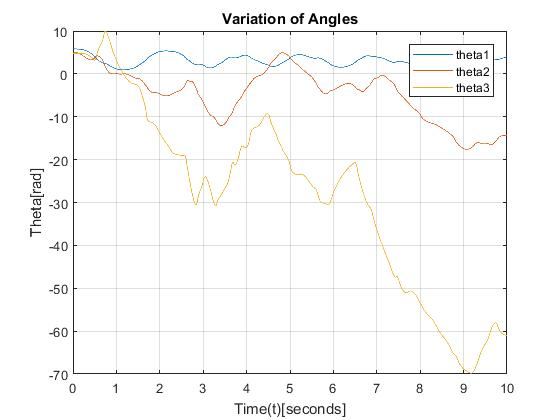
\includegraphics[width=1\linewidth]{theta.jpg}
\caption{Variation of ${\theta}$ for ${m_{1}=0.2944}$}\label{fig:theta_comp}
\end{subfigure}
\begin{subfigure}{0.5\textwidth}
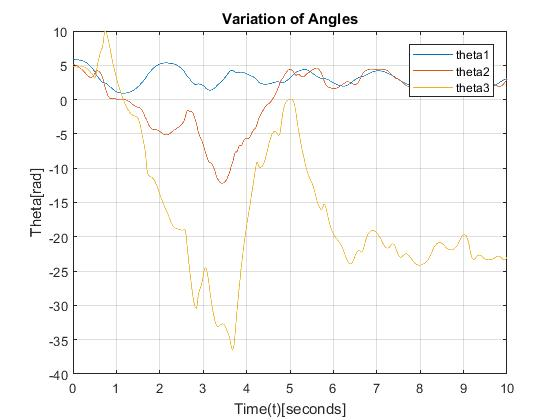
\includegraphics[width=1\linewidth]{theta_near.jpg}
\caption{Variation of ${\theta}$ for ${m_{1}=0.294401}$}\label{fig:trajectory_near_comp}
\end{subfigure}
\caption{Plot showing Sensitivity to Parameter value ${m}$ with ${\Delta m = 10^{-6}}$}\label{fig:image6}
\end{figure}

\begin{figure}[H]
\begin{subfigure}{0.5\textwidth}
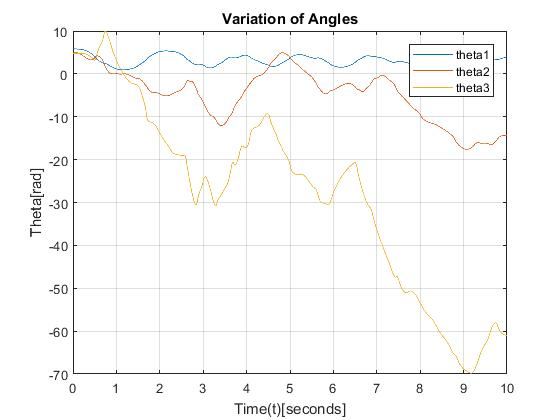
\includegraphics[width=1\linewidth]{theta.jpg}
\caption{Variation of ${\theta}$ for ${\theta_{1}(0)=-0.4603}$}\label{fig:theta_comp}
\end{subfigure}
\begin{subfigure}{0.5\textwidth}
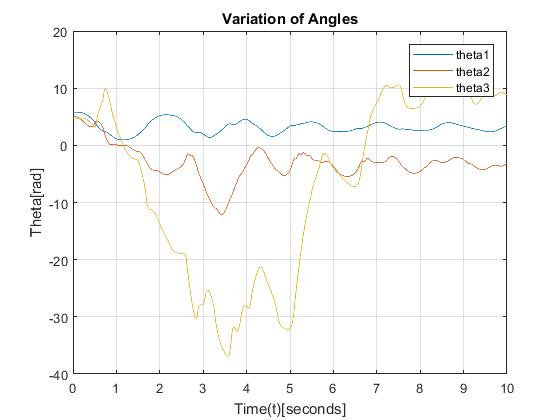
\includegraphics[width=1\linewidth]{theta_ch.jpg}
\caption{Variation of ${\theta}$ for ${\theta_{1}(0)=-0.460301}$}\label{fig:theta_ch_comp}
\end{subfigure}
\caption{Plot showing Sensitivity to Intital condition of ${\theta_{1}}$with ${\Delta \theta_{1} = 10^{-6}}$}\label{fig:image7}
\end{figure}

The proposed cryptosystem also holds such properties. The three qualities mentioned earlier are clearly evident from the plots and graphs shown Fig. 5.15 and Fig. 5.16. It is observed that keeping the parameters in one case and initial conditions in another case, constant leads to two completely different trajectories. Thus the map generated from the compound triple pendulum model possesses the essential chaotic properties to be employed in a general cryptosystem. 

\subsubsection{Collision Test}
Collision resistance is a property of cryptographic algorithms which makes it difficult to find two inputs which are encrypted to the same output. It must be ensured that finding collisions must be kept as hard as some of the hard mathematical problems like integer factorization  or discrete logarithm. Collision resistance does not mean that no collisions exist, it simply means that they are very hard to find. Here, we show that the proposed algorithm is fully collision resistant i.e. no collisions exist.

Since the entire range of $\theta$'s are partitioned according to the number of characters(say 256), different characters are mappped to points in different intervals. Hence two different inputs having different characters are completely mapped to different intervals. So the encryption scheme is completely free of collisions. 

\subsubsection{Test for Randomness}
For testing randomness of the chaotic map, necessary statistical tests were applied. These statistical tests are generally employed for testing randomness in pseudo random number generators. Here, Diehard random number generator test suite has been used to do such tests. Developed by George Marsaglia, Diehard is a battery of tests which are used to determine the quality of PRNGs. The list of tests performed on the generated chaotic map data and the corresponding results obtained are shown in Table 5.1.

\begin{table}[h!]
\begin{center}
\caption{Dieharder Test}
\label{tab:table1}
\begin{tabular}{|c|c|c|c|c|c|} % <-- Alignments: 1st column left, 2nd middle and 3rd right, with vertical lines in between
    \hline
    \textbf{test\_name} & \textbf{ntup} & \textbf{tsamples} & \textbf{psamples} & \textbf{p-value} & \textbf{Assessment}\\
    \hline
    diehard\_birthdays &    0 &        100 &      100 & 0.98409924 &   PASSED \\  
    diehard\_operm5 &    0 &    1000000 &      100 & 0.02570841 &   PASSED \\  
    diehard\_rank\_32x32 &    0 &      40000 &      100 & 0.30314396 &   PASSED \\  
    diehard\_rank\_6x8 &    0 &     100000 &      100 & 0.07586247 &   PASSED \\  
    diehard\_bitstream &    0 &    2097152 &      100 & 0.83264505 &   PASSED \\  
    diehard\_opso &    0 &    2097152 &      100 & 0.93701062 &   PASSED \\  
    diehard\_oqso &    0 &    2097152 &      100 & 0.63759752 &   PASSED \\  
    diehard\_dna &    0 &    2097152 &      100 & 0.73795350 &   PASSED \\  
    diehard\_count\_1s\_str &    0 &     256000 &      100 & 0.77268562 &   PASSED \\  
    diehard\_count\_1s\_byt &    0 &     256000 &      100 & 0.55542008 &   PASSED \\  
    diehard\_parking\_lot &    0 &      12000 &      100 & 0.70977074 &   PASSED \\  
    diehard\_2dsphere &    2 &       8000 &      100 & 0.58428028 &   PASSED \\  
    diehard\_3dsphere &    3 &       4000 &      100 & 0.86446205 &   PASSED \\  
    diehard\_squeeze &    0 &     100000 &      100 & 0.19422339 &   PASSED \\  
    diehard\_sums &    0 &        100 &      100 & 0.33263813 &   PASSED \\  
    diehard\_runs &    0 &     100000 &      100 & 0.50609448 &   PASSED \\    
    diehard\_craps &    0 &     200000 &      100 & 0.36377661 &   PASSED \\   
    marsaglia\_tsang\_gcd &    0 &   10000000 &      100 & 0.66121444 &   PASSED \\ 
    sts\_monobit &    1 &     100000 &      100 & 0.31074688 &   PASSED \\  
    sts\_runs &    2 &     100000 &      100 & 0.98606705 &   PASSED \\  
    sts\_serial &    1 &     100000 &      100 & 0.23629469 &   PASSED \\  
    sts\_serial &    2 &     100000 &      100 & 0.85410639 &   PASSED \\  
    sts\_serial &    8 &     100000 &      100 & 0.11131795 &   PASSED \\  
    sts\_serial &   16 &     100000 &      100 & 0.83380616 &   PASSED \\  
    rgb\_bitdist &    1 &     100000 &      100 & 0.45061356 &   PASSED \\  
    rgb\_bitdist &    6 &     100000 &      100 & 0.53111009 &   PASSED \\   
    rgb\_bitdist &   12 &     100000 &      100 & 0.64865649 &   PASSED \\  
    rgb\_minimum\_distance &    2 &      10000 &     1000 & 0.41755433 &   PASSED \\   
    rgb\_minimum\_distance &    4 &      10000 &     1000 & 0.11298477 &   PASSED \\  
    rgb\_permutations &    2 &     100000 &      100 & 0.79654377 &   PASSED \\ 
    rgb\_permutations &    4 &     100000 &      100 & 0.85371565 &   PASSED \\  
    rgb\_lagged\_sum &    0 &    1000000 &      100 & 0.92039997 &   PASSED \\   
    rgb\_lagged\_sum &   16 &    1000000 &      100 & 0.78219023 &   PASSED \\   
    rgb\_lagged\_sum &   32 &    1000000 &      100 & 0.64955712 &   PASSED \\  
    rgb\_kstest\_test &    0 &      10000 &     1000 & 0.58005862 &   PASSED \\  
    dab\_bytedistrib &    0 &   51200000 &        1 & 0.01089458 &   PASSED \\  
    dab\_dct &  256 &      50000 &        1 & 0.06122408 &   PASSED \\  
    dab\_filltree &   32 &   15000000 &        1 & 0.12524761 &   PASSED \\   
    dab\_filltree2 &    0 &    5000000 &        1 & 0.50605989 &   PASSED \\  
    dab\_monobit2 &   12 &   65000000 &        1 & 0.27940682 &   PASSED \\  
        
    \hline
\end{tabular}
\end{center}
\end{table}

It is observed that in most of the tests, the chaotic map generator performs well. This can be attributed largely due to the non-linear dynamics of the map.

\subsection{Complexity Analysis}

In this report, we give an overview of the computational complexity of the algorithm both on software as well as hardware level.

\subsubsection{Setup Complexity}
Firstly, the computation of the state variable (${\theta}$) values for a time duration $t$ and time step $\Delta t$ requires $N$ iterations where $N= \frac{t}{\Delta t}$. In each iteration only 6 equations are solved for the 6 state variables ($\theta_{1}, \theta_{2}, \theta_{3}, \dot{\theta_{1}}, \dot{\theta_{2}}, \dot{\theta_{3}}$) each in $O(1)$ time. Thus the time required for generating the map is asymptotically $O(N)$. Here space complexity is also $O(N)$ for storing the state variable values. Secondly, Baptista type patitioning takes constant time if the range of the variables are already computed in the previous step. For assigning the variable values to the corresponding intervals, $O(N)$ time is required for each value. Thirdly, for encryption of a plaintext having $M$ characters, there would be $M$ iterations and in each iteration the encrypted value is randomly selected from the computed interval which takes constant time. So the time complexity for setup of the encryption module is $O(N)$ and $O(M)$ is the time complexity of processing each plaintext. Space complexity is still $O(N)$. Similarly, for decryption time complexity is also $O(N)$ and $O(M)$ for setup and processing respectively.\\
\textbf{Information Rate:} The information rate of any cryptosysytem is define d as the ratio of the size of plaintext to that of the cipher text. In our cryptosystem, we have
\begin{equation}
R = \frac{plaintext\ size}{ciphertext\ size} = \frac{8*M}{\log_2N*M} = \frac{8}{\log_2N}
\end{equation}
\subsubsection{Hardware Resource Utilization}
The following (Fig. 5.17) shows the resource utilization of the complete RTL implementation after synthesis using XST tool. The maximum resources used is in the storage of state variable values in the LUT. It is only about 1.3\% of the total fgpa memory and hence the memory usage is quite low. It can be seen that 1726 LUTs and 1883 Flip-Flops are required. Also, due to target device being FPGA, instances of DSP48 have been used.
\begin{figure}[H]
\centering
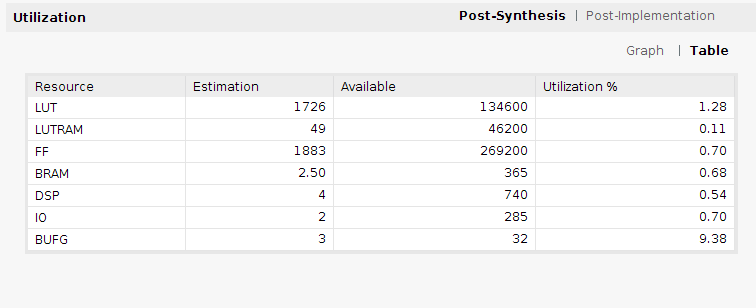
\includegraphics[width=0.7\linewidth]{table.png}
\caption{Table showing Resource Utilization}\label{fig:table}
\end{figure}

% \begin{figure}[H]
% \centering
% 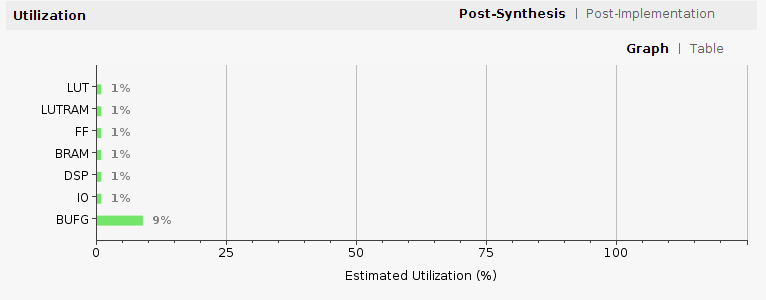
\includegraphics[width=0.4\linewidth]{graph.png}
% \caption{Bar graph showing Resource Utilization}\label{fig:graph}
% \end{figure}

\subsection{Reason for being Quantum-Safe}
The argument in regards to the quantum-safe property of this algorithm is due to its innate chaotic nature. Traditional Shor's and Glover's algorithms cannot break this system as they deal with a different paradigm of hard problems like integer factorization and discrete logarithm. Also the highly non-linear and interdependent nature of the dynamical system makes it difficult for even the quantum algorithms to do brute force attacks without the total or partial knowledge of key. Even with partial knowledge of key values, it is useless to do brute force attacks as the chaotic maps are highly sensitive to key values. The key size is about $21\times(32 bits) = 672 bits$ for single precision arithmetic which is quite large enough. All these reasons direct us to be confidently stand by this algorithms and call it quantum computing immune. 
